% Options for packages loaded elsewhere
\PassOptionsToPackage{unicode}{hyperref}
\PassOptionsToPackage{hyphens}{url}
\PassOptionsToPackage{dvipsnames,svgnames,x11names}{xcolor}
%
\documentclass[
  letterpaper,
  DIV=11,
  numbers=noendperiod]{scrreprt}

\usepackage{amsmath,amssymb}
\usepackage{iftex}
\ifPDFTeX
  \usepackage[T1]{fontenc}
  \usepackage[utf8]{inputenc}
  \usepackage{textcomp} % provide euro and other symbols
\else % if luatex or xetex
  \usepackage{unicode-math}
  \defaultfontfeatures{Scale=MatchLowercase}
  \defaultfontfeatures[\rmfamily]{Ligatures=TeX,Scale=1}
\fi
\usepackage{lmodern}
\ifPDFTeX\else  
    % xetex/luatex font selection
\fi
% Use upquote if available, for straight quotes in verbatim environments
\IfFileExists{upquote.sty}{\usepackage{upquote}}{}
\IfFileExists{microtype.sty}{% use microtype if available
  \usepackage[]{microtype}
  \UseMicrotypeSet[protrusion]{basicmath} % disable protrusion for tt fonts
}{}
\makeatletter
\@ifundefined{KOMAClassName}{% if non-KOMA class
  \IfFileExists{parskip.sty}{%
    \usepackage{parskip}
  }{% else
    \setlength{\parindent}{0pt}
    \setlength{\parskip}{6pt plus 2pt minus 1pt}}
}{% if KOMA class
  \KOMAoptions{parskip=half}}
\makeatother
\usepackage{xcolor}
\setlength{\emergencystretch}{3em} % prevent overfull lines
\setcounter{secnumdepth}{5}
% Make \paragraph and \subparagraph free-standing
\ifx\paragraph\undefined\else
  \let\oldparagraph\paragraph
  \renewcommand{\paragraph}[1]{\oldparagraph{#1}\mbox{}}
\fi
\ifx\subparagraph\undefined\else
  \let\oldsubparagraph\subparagraph
  \renewcommand{\subparagraph}[1]{\oldsubparagraph{#1}\mbox{}}
\fi


\providecommand{\tightlist}{%
  \setlength{\itemsep}{0pt}\setlength{\parskip}{0pt}}\usepackage{longtable,booktabs,array}
\usepackage{calc} % for calculating minipage widths
% Correct order of tables after \paragraph or \subparagraph
\usepackage{etoolbox}
\makeatletter
\patchcmd\longtable{\par}{\if@noskipsec\mbox{}\fi\par}{}{}
\makeatother
% Allow footnotes in longtable head/foot
\IfFileExists{footnotehyper.sty}{\usepackage{footnotehyper}}{\usepackage{footnote}}
\makesavenoteenv{longtable}
\usepackage{graphicx}
\makeatletter
\def\maxwidth{\ifdim\Gin@nat@width>\linewidth\linewidth\else\Gin@nat@width\fi}
\def\maxheight{\ifdim\Gin@nat@height>\textheight\textheight\else\Gin@nat@height\fi}
\makeatother
% Scale images if necessary, so that they will not overflow the page
% margins by default, and it is still possible to overwrite the defaults
% using explicit options in \includegraphics[width, height, ...]{}
\setkeys{Gin}{width=\maxwidth,height=\maxheight,keepaspectratio}
% Set default figure placement to htbp
\makeatletter
\def\fps@figure{htbp}
\makeatother
% definitions for citeproc citations
\NewDocumentCommand\citeproctext{}{}
\NewDocumentCommand\citeproc{mm}{%
  \begingroup\def\citeproctext{#2}\cite{#1}\endgroup}
\makeatletter
 % allow citations to break across lines
 \let\@cite@ofmt\@firstofone
 % avoid brackets around text for \cite:
 \def\@biblabel#1{}
 \def\@cite#1#2{{#1\if@tempswa , #2\fi}}
\makeatother
\newlength{\cslhangindent}
\setlength{\cslhangindent}{1.5em}
\newlength{\csllabelwidth}
\setlength{\csllabelwidth}{3em}
\newenvironment{CSLReferences}[2] % #1 hanging-indent, #2 entry-spacing
 {\begin{list}{}{%
  \setlength{\itemindent}{0pt}
  \setlength{\leftmargin}{0pt}
  \setlength{\parsep}{0pt}
  % turn on hanging indent if param 1 is 1
  \ifodd #1
   \setlength{\leftmargin}{\cslhangindent}
   \setlength{\itemindent}{-1\cslhangindent}
  \fi
  % set entry spacing
  \setlength{\itemsep}{#2\baselineskip}}}
 {\end{list}}
\usepackage{calc}
\newcommand{\CSLBlock}[1]{\hfill\break\parbox[t]{\linewidth}{\strut\ignorespaces#1\strut}}
\newcommand{\CSLLeftMargin}[1]{\parbox[t]{\csllabelwidth}{\strut#1\strut}}
\newcommand{\CSLRightInline}[1]{\parbox[t]{\linewidth - \csllabelwidth}{\strut#1\strut}}
\newcommand{\CSLIndent}[1]{\hspace{\cslhangindent}#1}

\KOMAoption{captions}{tableheading}
\makeatletter
\@ifpackageloaded{bookmark}{}{\usepackage{bookmark}}
\makeatother
\makeatletter
\@ifpackageloaded{caption}{}{\usepackage{caption}}
\AtBeginDocument{%
\ifdefined\contentsname
  \renewcommand*\contentsname{Table of contents}
\else
  \newcommand\contentsname{Table of contents}
\fi
\ifdefined\listfigurename
  \renewcommand*\listfigurename{List of Figures}
\else
  \newcommand\listfigurename{List of Figures}
\fi
\ifdefined\listtablename
  \renewcommand*\listtablename{List of Tables}
\else
  \newcommand\listtablename{List of Tables}
\fi
\ifdefined\figurename
  \renewcommand*\figurename{Figure}
\else
  \newcommand\figurename{Figure}
\fi
\ifdefined\tablename
  \renewcommand*\tablename{Table}
\else
  \newcommand\tablename{Table}
\fi
}
\@ifpackageloaded{float}{}{\usepackage{float}}
\floatstyle{ruled}
\@ifundefined{c@chapter}{\newfloat{codelisting}{h}{lop}}{\newfloat{codelisting}{h}{lop}[chapter]}
\floatname{codelisting}{Listing}
\newcommand*\listoflistings{\listof{codelisting}{List of Listings}}
\makeatother
\makeatletter
\makeatother
\makeatletter
\@ifpackageloaded{caption}{}{\usepackage{caption}}
\@ifpackageloaded{subcaption}{}{\usepackage{subcaption}}
\makeatother
\ifLuaTeX
  \usepackage{selnolig}  % disable illegal ligatures
\fi
\usepackage{bookmark}

\IfFileExists{xurl.sty}{\usepackage{xurl}}{} % add URL line breaks if available
\urlstyle{same} % disable monospaced font for URLs
\hypersetup{
  pdftitle={APP-WASM-summative},
  pdfauthor={Alison Harper},
  colorlinks=true,
  linkcolor={blue},
  filecolor={Maroon},
  citecolor={Blue},
  urlcolor={Blue},
  pdfcreator={LaTeX via pandoc}}

\title{APP-WASM-summative}
\author{Alison Harper}
\date{2025-08-05}

\begin{document}
\maketitle

\renewcommand*\contentsname{Table of contents}
{
\hypersetup{linkcolor=}
\setcounter{tocdepth}{2}
\tableofcontents
}
\bookmarksetup{startatroot}

\chapter*{Preface}\label{preface}
\addcontentsline{toc}{chapter}{Preface}

\markboth{Preface}{Preface}

Summative assessment for APP.

WebAssembly has been proposed as a suitable approach for supporting NHS
operational decision-making using discrete event simulation. It enables
NHS users to interact with a model locally, meaning sensitive data is
only used locally, with no risk of data breaches.

This project explores its applicability to education, specifically for
learning about simulation modelling as a method of supporting
operational, strategic, and supply chain resourcing, planning, and
configuring.

\bookmarksetup{startatroot}

\chapter{WebAssembly for discrete event
simulation}\label{webassembly-for-discrete-event-simulation}

\section{WebAssembly for discrete-event simulation using
Python:}\label{webassembly-for-discrete-event-simulation-using-python}

\section{Teaching-Research Synergy}\label{teaching-research-synergy}

The use of WebAssembly has significant implications for the deployment
of healthcare simulation models for NHS staff use, to support planning
their services. It overcomes many of the issues of other methods of
deployment, by increasing accessibility, usability, and data security.
It also has the potential to address some of the challenges faced for
simulation education, which include usability and democratisation of
access. The learnings from use in the healthcare sector are proposed to
be transferable to education.

\subsection{\texorpdfstring{\textbf{1. Discrete-event Simulation as a
method}}{1. Discrete-event Simulation as a method}}\label{discrete-event-simulation-as-a-method}

In everyday life we encounter the concept of simulation. Weather apps
simulate patterns of rainfall and atmosphere dynamics over the coming
hours and days. Simulations help understand how diseases or pollutants
spread. Urban planners use simulation to study traffic patterns and plan
road layouts, or flood risks to plan new developments.

Discrete-event simulation (DES) is a type of computer simulation used to
model the operation of complex systems, as a sequence of discrete events
in time. Events might be arrivals, departures, starting or ending of
services, or failures or repairs of resources. Many systems modelled
using DES involve queues or delays, so processes are often modelled in
terms of a series of queues and servers. As events usually occur at
random times, and may have random effects, simulation incorporates
elements of probability to reflect this real-life randomness.

A DES model can be seen as a computer representation of a system.
Running it over time replicates the behaviour of the system over time.
Simulation is often used where research on the real system is not
possible, due to inaccessibility, risks, or costs. Experimentation with
the simulation model is used instead of experimenting with the real
system.

\subsection{\texorpdfstring{\textbf{2. Research
focus}}{2. Research focus}}\label{research-focus}

\subsubsection{2.1 Reuse of simulation models in
healthcare}\label{reuse-of-simulation-models-in-healthcare}

DES models are widely used for decision-support in healthcare, for
example for demand and capacity planning of health services. However,
they are time-consuming to develop for both modellers and healthcare
stakeholders, and are often treated as disposable artefacts, once
results have been analysed and delivered. Additionally, for healthcare
M\&S researchers, a long-standing challenge is translating model results
into real-world practice. While many factors contribute to successful
model uptake, the aim is to overcome some of the barriers to model use
in healthcare by enabling healthcare decision-makers to access and use
the model.

Across healthcare services, similar problems are seen in similar
application areas. Model reuse is seen as a potential solution to reduce
duplication of effort and maximise the potential value gained from the
model. Model reuse can involve re-developing, modifying, or
reparaterising an existing model. Another approach to model reuse is to
deploy a simulation model for the same purpose in a single application
area, which can be used repeatedly for planning by healthcare staff such
as managers, clinicians or analysts.

A model deployed for reuse by healthcare stakeholders needs to be
available and accessible. Purpose built software can make this easy, but
may come with prohibitive licensing arrangements and costs. While Python
democratises the availability of software, and with appropriate open
licensing, allows models to be freely shared and adapted, programming
languages such as Python can present accessibility and usability
challenges for non-technical users, who may most benefit from their use.

\subsubsection{2.2 Simulation model deployment
options}\label{simulation-model-deployment-options}

Model deployment refers to the process of taking a validated DES model
and making it available for use in real-world applications. It
transitions a model from a development setting, where it is tested and
validated, to an operational setting where it can provide practical
value.

The choice of deployment method should be tailored to fit the specific
needs of stakeholders and the user-base within a project, as different
methods of deployment come with advantages and disadvantages.

Using Jupyter, models, including their source code, can be deployed as
static files, interactive web pages, or hosted on platforms like GitHub,
Binder, or Google Colab. They can also be shared as web apps, with
user-friendly interfaces, via free platforms such as Streamlit Community
Cloud. While these are convenient ways to share a model, free or
limited-capacity platforms restrict the number of processors available,
memory, and/or bandwidth. Some, such as ShinyApps, offer monthly paid
plans to increase computational resources, which may not be budgeted
into a project. In healthcare, a bigger issue is the potential need to
use sensitive data or parameters, which may require a private, local
instance of a model where model parameters/data are not sent to any
remote servers, so server vulnerabilities are mitigated.

A standard approach is to commit code and virtual environments files to
GitHub (or alternative repository) which can then be downloaded and run
locally. Using Conda environments allows for a controlled setup that
maintains dependencies without complex configurations. For NHS users
with limited technical support, this can present barriers. WebAssembly
is an alternative approach for local processing which eliminates the
need for complex software installation processes. Input files are used
locally, and output files and data be safely exported to the users
laptop or desktop. Additionally, every user accesses the same software
environment directly in their browser, ensuring consistency,
reliability, and reproducibility of model results.

\subsubsection{2.2.1 Models as Notebooks: Jupyter and
JupyterLite}\label{models-as-notebooks-jupyter-and-jupyterlite}

Jupyter Notebooks and Jupyterlab provide a web-based interactive
computing platform which allows users to create and share `notebooks',
which execute code, equations, visualisations and narrative text in a
step-by-step manner. This is particularly beneficial for data analysis,
prototyping, and education.

\begin{figure}[H]

{\centering 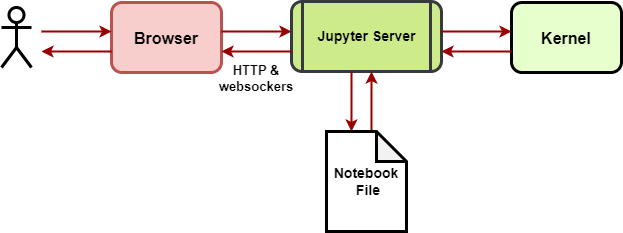
\includegraphics{notebooks/images/Normal_jupyter2.drawio.png}

}

\caption{Jupyter architecture}

\end{figure}%

Using WebAssembly, JupyterLite is a lightweight version of Jupyter that
runs entirely in the browser without the need for server-side
infrastructure. Jupyter notebooks can be created and run locally without
installing anything on their machines. It is fast, portable, and easily
deployable, making it ideal for lightweight computing tasks and
educational purposes.

Figure 2: JupyterLite architecture

\subsubsection{2.2.2 Models with an interface: Streamlit and
Stlite}\label{models-with-an-interface-streamlit-and-stlite}

Streamlit is a Python library that allows modellers to quickly create
interactive web applications for their DES models, and other data
science projects. It simplifies the process of building custom web
interfaces by providing easy-to-use widgets and tools for changing
simulation parameters and visualising data.

Figure 3: Streamlit architecture

Stlite is a WebAssembly implementation of Streamlit, enabling the
creation of web applications using Python syntax, but compiled to run in
the browser. This allows for building interactive DES models without the
need for a server backend. It is fast and flexible, and ideal for
lightweight tasks such as enabling NHS stakeholders to access and use a
model. It is particularly suitable for rapid prototyping during a
project, and for ease-of-use after a project end.

Figure 4: Stlite architecture

\subsection{\texorpdfstring{\textbf{3. Summary of deploying models for
healthcare
research}}{3. Summary of deploying models for healthcare research}}\label{summary-of-deploying-models-for-healthcare-research}

In healthcare, reusable models have the potential to increase the impact
of a modelling and simulation study, by making models available for
direct use by NHS stakeholders. Attention needs to be given to deploying
models that are accessible, usable, and functional in line with the
needs of non-technical stakeholders. However, healthcare models also
need to focus on security of sensitive data, and WebAssembly of code
notebooks or model interfaces addresses this issue with client-side
execution

\bookmarksetup{startatroot}

\chapter{}\label{section}

\bookmarksetup{startatroot}

\chapter{Summary}\label{summary}

In summary, this book has no content whatsoever.

\bookmarksetup{startatroot}

\chapter*{References}\label{references}
\addcontentsline{toc}{chapter}{References}

\markboth{References}{References}

\phantomsection\label{refs}
\begin{CSLReferences}{0}{1}
\end{CSLReferences}



\end{document}
